\section{算法层创新}

现有问题在于：原始 DynamicViT 的词元删除、阈值比较与数据相关 Top-选择依赖明文控制流，直接迁入安全计算图会同时遭遇变长结构、路径泄露和并列分数不稳定三类困难，因此常见方案通常选择放弃动态剪枝，退回固定结构安全推理。

本作品的做法是把 pruning boundary 从“删除式表达”重写为“掩码化表达”，将词元保留决策改写为基于安全选择原语的  表达，将阈值判断改写为基于安全比较原语的  表达，并结合编码键双调排序（Encoded-Key Bitonic Sort）处理安全 Top-（前选择）与并列分数决断问题。这样做的意义在于，不仅让动态剪枝能够进入固定图安全执行环境，而且保留了按样本变化的剪枝决策能力，而不是用一个固定结构模型替代原始方法。

这一层的技术难点在于：既要避免数据相关分支泄露，又要在固定图语义下近似保留原始动态模型的判别边界；同时，排序与并列分数处理必须在安全执行环境内稳定完成，否则最终决策链会因 tie 或索引不稳定而失去可验证性。

实验证据表明，该改写并未使动态路径退化为不可部署状态：动态安全剪枝链路相较固定结构静态对照线的阈值精度提升 0.7634 个百分点，相较未经安全化边界重写的原始 DynamicViT 提升 17.3664 个百分点。该层内容由第 2.4 节密态改写表、第 4.2 节基线对比、第 4.3 节医疗结果与第 4.7 节结果分析共同支撑。第四章的消融结果进一步说明，该创新并非“只是在安全执行域中复现一条既有推理链”，而是实质性保留了动态剪枝在部署口径下的有效判别边界：去掉动态剪枝后，阈值精度由92.7481\%下降至89.6947\%，AUC由0.9639下降至0.9539，表明动态剪枝安全化改写对最终可部署性能具有直接贡献。

\section{系统层创新}

现有问题在于，不少安全推理系统虽然使用了密态执行框架，但会在外部明文环境中预先决定剪枝路径，再把结果送入密态推理后端。这类做法虽然降低了工程难度，却使动态状态、路径信息甚至部分模型行为暴露在安全执行域之外，本质上仍属于半隐私运行。

本作品的做法是将动态剪枝预测器 PredictorLG、阈值判断与并列分数决断保留在安全执行域内，并以 SPU 与 OpenBumbleBee 组成两方安全计算链路，对输入数据、模型参数和中间动态决策状态同时进行保护。这样，系统不再依赖“外部先算路径、内部只回放”的简化策略，而是在双向隐私前提下完成完整的动态决策链执行。

这一层的技术难点在于：既要在两方半诚实模型下维持输入与参数的双向隐私边界，又要让动态路径的关键控制流保留在密态环境内执行；如果处理不当，系统很容易退化为只保护输入或只保护模型的单向隐私方案。

实验证据方面，当前端到端原型在 32 条医疗部署验证样本上的双向总通信量为 84.47 GiB，且服务端不接收明文像素值、模型参数不以明文暴露，对外仅返回最终分类结果；金融边界压力样本 8/8 与明文参考逐样本一致。该层内容由第 2.1 节总体架构、第 2.2 节威胁模型与安全边界、第 3.1 节两方安全推理链路、第 4.3 节医疗结果与第 4.5 节金融边界验证共同支撑。

\section{工程层特色与可验证交付能力}

现有问题在于，很多 Web 演示只展示模型输出结果，默认将输入视为天然可信，缺少协议层异常输入阻断、审计链、资源状态回落记录和可复现实验入口。对于信息安全类作品而言，这类展示很难支撑“系统已形成工程闭环”的判断。

本作品的做法是把浏览器工作线程、本地数据质量评估、审计哈希链、服务端权威快检、协议层异常输入模糊测试、重放与并发守卫一起纳入交付范围。这里的重点不是把工程实现拔高为核心算法创新，而是使系统不仅能给出分类结果，还能证明输入经过了哪些检查、异常请求在何处被阻断，以及资源状态是否回到稳态。

这一层的技术难点在于：前端要在不阻塞主线程的前提下完成高开销预处理与审计摘要生成，服务端要在进入 SPU 前完成原始报文、JSON 元数据、share 字节流和张量层的多级快检，同时还要把异常输入、重放与并发探针的结果转化为可复核的证据文件。

实验证据方面，本作品已覆盖 17 类协议层与控制面黑盒用例，17/17 按预期返回，且采样窗口内未观察到文件描述符或套接字文件描述符净增长；同时仓内提供 10–20 分钟最低可复现路径，用于复核完整计算链路。该层内容由第 3.3 节前端控制面、第 3.4 节服务端权威快检与审计、第 4.6 节鲁棒性矩阵、第 6.1 节复现路径和 \texttt{README\textbackslash\{\}\_REPRODUCE.md} 共同支撑。

\section{与常见方案对比}

\begin{longtable}{>{\raggedright\arraybackslash}p{0.32\textwidth}>{\raggedright\arraybackslash}p{0.32\textwidth}>{\raggedright\arraybackslash}p{0.32\textwidth}}
\caption{表 14 本作品与常见隐私推理方案能力对比}\\
\toprule
\textbf{对比对象} & \textbf{常见做法} & \textbf{本作品差异} \\
\midrule
\endfirsthead
\toprule
\textbf{对比对象} & \textbf{常见做法} & \textbf{本作品差异} \\
\midrule
\endhead
固定结构安全推理 & 放弃动态剪枝，直接改为固定结构模型 & 保留按样本变化的剪枝决策，并把边界重写为可密态执行语义 \\
明文剪枝 + 密态推理 & 外部明文环境先决定路径，密态后端仅回放结果 & 剪枝决策链保留在安全执行域内完成，避免半隐私运行 \\
单向隐私推理 & 只保护输入或只保护模型参数 & 同时保护输入数据、模型参数和动态中间状态 \\
普通 Web 演示 & 只展示结果页面，不提供输入守卫与异常验证 & 加入服务端快检、审计链、模糊测试与重放/并发守卫证据 \\
\bottomrule
\end{longtable}

本作品与常见隐私推理方案在核心能力上的差异对比如表 14 所示。这组对比说明，本作品的主要价值不在于简单地“再做一条安全推理链”，而在于同时解决了动态剪枝保留、双向隐私成立、动态决策链不外泄以及工程交付可验证四个问题。若从已有隐私保护 ViT 路线来看，SViT[13] 代表的是“保持原始 ViT-B/16 结构不变，通过秘密共享安全协议优化降低推理开销”的方案。其优势在于协议边界清晰、非线性算子设计完整，并且在计算效率和在线通信量方面相较 CrypTen[16] 取得了较明显改善。相比之下，本作品的重点不在于复现固定结构 ViT 的安全执行，而在于把 DynamicViT 中原本依赖明文控制流的动态词元剪枝路径，重写为固定图下可执行的安全比较与安全选择语义，并进一步纳入浏览器端控制面、服务端权威快检和审计闭环。换言之，SViT 更偏向“协议优化型”隐私推理框架，而本作品更偏向“动态结构安全化 + 双向隐私 + 工程闭环”的综合方案。

为避免“文字对比结论”显得过于抽象，图 5-1 进一步把固定结构安全推理、明文剪枝后密态回放、单向隐私推理与本作品放在同一能力矩阵下进行边界比较。该图服务于第 5.4 节的总结性结论：本作品的差异不在于单独强化某一侧能力，而在于把动态剪枝、双向隐私、服务端权威快检与可复核控制面整合进同一条工程闭环。

\begin{figure}[htbp]
\centering
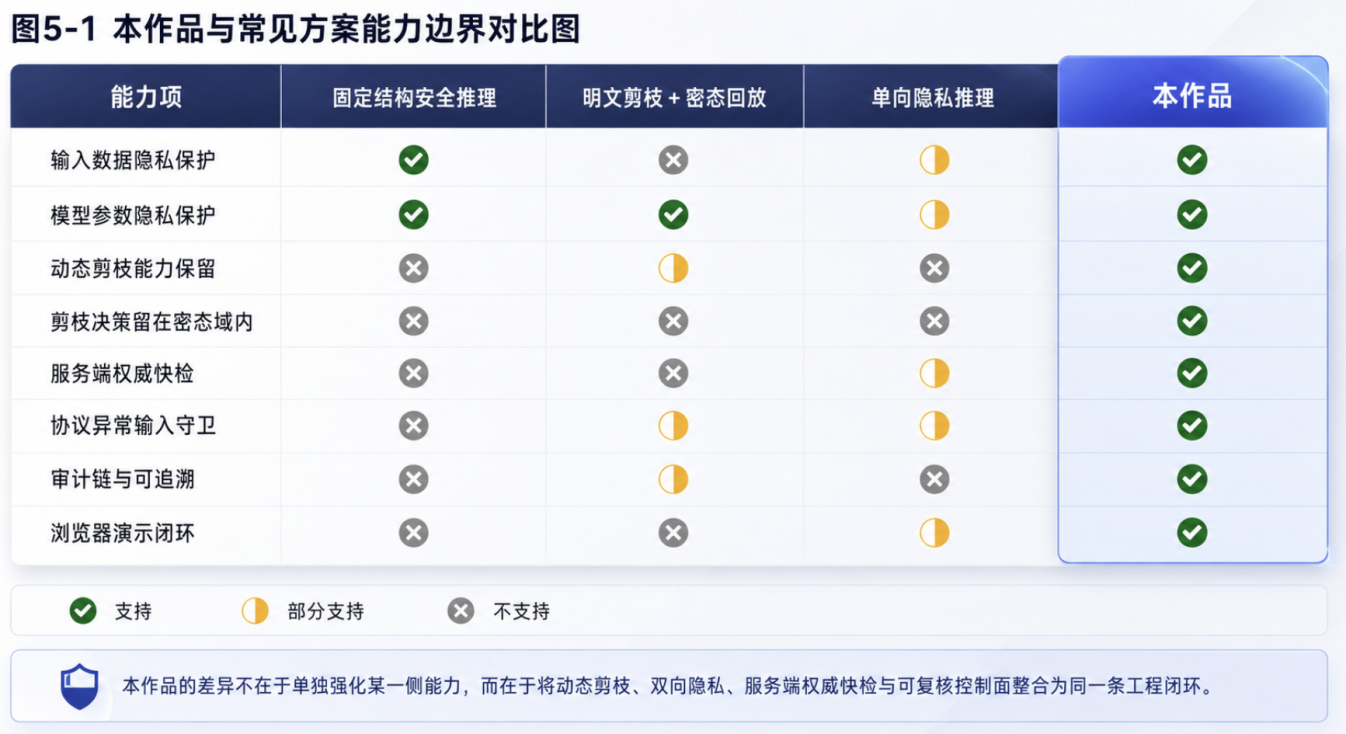
\includegraphics[width=0.92\textwidth]{figures/fig5-1-capability-matrix.jpeg}
\caption{图5-1 本作品与常见方案能力边界对比图：从动态剪枝、双向隐私、服务端快检与可追溯控制面四个维度展示差异。}
\end{figure}

如果把相关方案进一步分类，SecureML[14]、GAZELLE[15]、CrypTen[16] 与 Delphi[17] 更接近通用私有推理系统，它们为线性层、激活函数与模型服务接口提供基础协议与系统支撑；Iron[18]、BOLT[19]、BumbleBee[7] 与 NEXUS[20] 则代表固定结构 Transformer 的协议优化路线，重点降低注意力与非线性算子的执行成本；CipherPrune[21] 进一步把密态词元剪枝与多项式降阶结合起来，试图同时减少后续层 token 规模与近似开销。相比之下，本作品面向的是医疗影像 DynamicViT 场景，强调在两方半诚实模型下保留动态剪枝决策、明确服务端权威快检与审计边界，并为后续医院/模型提供方分离部署保留工程骨架。

从方法边界看，本作品目前选择的是“保留 DynamicViT 语义并进行安全化改写”的路线，而不是重新训练一套专门面向私有推理的 Transformer。其优点是能够直接解释作品与原始动态剪枝模型之间的关系，便于复现和工程交付；限制在于，固定图 keep-mask、排序网络和密态比较会带来额外开销，且尚未利用 CipherPrune[21]、THE-X[22]、MPCFormer[23]、SecFormer[24] 等工作中更激进的多项式化、蒸馏或结构替换策略。因此，当前方案更适合作为可运行的动态安全剪枝基线，而不是效率上限。

\section{当前局限性}

本作品当前仍有六点需要明确说明的边界。第一，当前展示后端采用单进程 Uvicorn/FastAPI 原型承载长耗时 SPU 调用，进入长耗时 SPU 计算后的主动断连感知、任务取消和队列化调度能力仍不完整，因此现有并发守卫不能等价替代生产级拒绝服务防护。第二，当前仓内仅固化了端到端通信量与算子级代理基准证据，未单独落盘医疗动态安全剪枝链路的阶段级时延剖面，因此尚不能给出更细粒度的性能分解。第三，金融任务当前只覆盖 8 条边界压力样本，足以支撑稳定性验证，但不足以单独构成第二应用主线。第四，当前安全模型主要建立在两方半诚实假设上，不覆盖恶意参与方串谋、模型抽取和更强侧信道对抗场景。第五，当前系统尚未系统评估输出结果本身可能带来的反推风险，因此输出侧隐私仍需在后续工作中单独建模与验证。第六，SViT 这类外部对照方案虽然在协议级性能方面表现较优，但仍依赖可信第三方和固定两方执行模型，说明当前隐私保护 ViT 系统在部署角色、信任假设和执行形态上仍存在约束。

此外，当前动态安全剪枝链路虽然已经证明 DynamicViT 安全化重写的可行性，但尚未在统一数据、统一硬件和统一执行边界下系统比较 Iron[18]、BOLT[19]、NEXUS[20]、CipherPrune[21] 等路线的全部收益差异。这意味着本作品当前更适合作为面向医疗影像动态剪枝场景的工程基线，而不是对所有私有 Transformer 方案给出普适最优结论。后续若要充分吸收密态渐进剪枝或非交互协议等新思路，还需要同步调整 keep-mask 生成策略、训练目标、近似算子和部署验证链路。
